% --- IMPORTS ---
\documentclass[leqno]{article}
\usepackage{graphicx}
\usepackage{dsfont}
\usepackage{mathtools}
\usepackage{amssymb}
\usepackage{amsmath}
\usepackage{amsthm}
\usepackage{float}
\usepackage{ragged2e}
\usepackage{tensor}
\usepackage{fancyhdr}
\usepackage{empheq}
\usepackage[most]{tcolorbox}
\usepackage{enumitem}
\usepackage{dirtytalk}
\usepackage{marginnote}
\usepackage{microtype}
\usepackage[
  a4paper,
  left=0.8in,
  right=1in,
  top=1in,
  bottom=0.5in,
  headheight=14pt,
  headsep=0.4in
]{geometry}
\setlength{\parindent}{0cm}
% --- TikZ Packages ---
\usepackage{pgfplots}
\pgfplotsset{compat=1.18}
\usepgfplotslibrary{fillbetween, polar}
\usetikzlibrary{calc, positioning}
\usetikzlibrary{angles, quotes}
\usetikzlibrary{arrows.meta}
\usetikzlibrary{decorations.pathreplacing, decorations.markings}
\usetikzlibrary{patterns}
\usetikzlibrary{intersections}
% --- URL Packages ---
\usepackage[colorlinks=true,linkcolor=red,citecolor=magenta,urlcolor=black]{hyperref}%
\urlstyle{same}
% --- END OF IMPORTS ---

% --- CUSTOM COMMANDS ---
\RenewDocumentCommand{\marks}{o m}{%
  \IfValueTF{#1}%
    {\marginnote{\raggedright\textbf{[#2]}}[#1]}%
    {\marginnote{\raggedright\textbf{[#2]}}}%
}
\newcommand{\vspacerule}[2]{%
  \par\vspace*{#1}%
  \noindent\hrulefill\par
  \vspace*{#2}%
}
\definecolor{scarlet}{RGB}{205, 40, 75}
\newcommand{\questionitem}{%
  \item\phantomsection
  \addcontentsline{toc}{section}{Question \number\value{enumi}}%
}
\renewcommand{\contentsname}{Questions}
% --- END OF CUSTOM COMMANDS ---

% --- HEADER CONFIG ---
\pagestyle{fancy}
\fancyhead{}
\fancyfoot{}
\renewcommand{\headrulewidth}{0.9pt}
\lhead{\textit{Solutions} - Vector Momentum and Impulse}
\chead{}
\rhead{\href{https://danieljsmith.org}{danieljsmith.org}}
% --- END OF HEADER CONFIG ---

\begin{document}
\vspace*{20pt}
\tableofcontents
\newpage
\begin{enumerate}[
  label=\textbf{\arabic*.},
  leftmargin=*,
  topsep=0pt,
  partopsep=0pt,
  parsep=0pt
]

% ---- Question 1 ----
\questionitem
% [Source: _QBT__Vector_Momentum_and_Impulse, Q1]

A particle $P$ of mass $2\,\mathrm{kg}$ is moving with speed $15\,\mathrm{m\,s^{-1}}$ in the direction of $3\mathbf{i}+4\mathbf{j}$ when it receives an impulse $\mathbf{J}\,\mathrm{N\,s}$. Immediately after receiving the impulse, $P$ is moving with speed $17\,\mathrm{m\,s^{-1}}$ in the direction of $8\mathbf{i}+15\mathbf{j}$. \\

\begin{enumerate}[label=\textbf{(\alph*)}]
  \item Find the magnitude of $\mathbf{J}$ \marks{4} \\
\end{enumerate}
The angle between the direction of the impulse and the direction of motion of $P$ immediately before receiving the impulse is $\alpha^\circ$. \\
\begin{enumerate}[label=\textbf{(\alph*)}, resume]
  \item Find the value of $\alpha$ \marks{3} \\
\end{enumerate}

\vspace*{10pt}

\begin{tcolorbox}[colback=white, colframe=scarlet, title={\textbf{Solution}}, breakable, grow to left by=6mm, grow to right by=10mm]
\begin{enumerate}[label=\textbf{(\alph*)}]
  \item The initial direction is $3\mathbf{i}+4\mathbf{j}$, whose magnitude is
  \[
  \sqrt{3^2+4^2}=5
  \]
  So the initial velocity is
  \[
  \mathbf{u}=15\left(\frac{3\mathbf{i}+4\mathbf{j}}{5}\right)=9\mathbf{i}+12\mathbf{j}
  \]

  The final direction is $8\mathbf{i}+15\mathbf{j}$, whose magnitude is
  \[
  \sqrt{8^2+15^2}=17
  \]
  So the final velocity is
  \[
  \mathbf{v}=17\left(\frac{8\mathbf{i}+15\mathbf{j}}{17}\right)=8\mathbf{i}+15\mathbf{j}
  \]

  Using impulse $=$ change in momentum,
  \[
  \mathbf{J}=2(\mathbf{v}-\mathbf{u})
  \]
  Hence
  \begin{align*}
  \mathbf{J}
  &=2\bigl((8-9)\mathbf{i}+(15-12)\mathbf{j}\bigr) \\
  &=2(-\mathbf{i}+3\mathbf{j}) \\
  &=-2\mathbf{i}+6\mathbf{j}
  \end{align*}

  Therefore its magnitude is
  \begin{align*}
  |\mathbf{J}|
  &=\sqrt{(-2)^2+6^2} \\
  &=\sqrt{40} \\
  &=2\sqrt{10}
  \end{align*}

  So the magnitude of the impulse is $2\sqrt{10}\,\mathrm{N\,s}$.

  \item The direction of motion before the impulse is the direction of $3\mathbf{i}+4\mathbf{j}$.

  The impulse vector is
  \[
  \mathbf{J}=-2\mathbf{i}+6\mathbf{j}
  \]
  Let $\alpha$ be the angle between $\mathbf{J}$ and $3\mathbf{i}+4\mathbf{j}$.

  Using the scalar product,
  \[
  \cos\alpha=\frac{\mathbf{J}\cdot(3\mathbf{i}+4\mathbf{j})}{|\mathbf{J}|\cdot|3\mathbf{i}+4\mathbf{j}|}
  \]
  Now
  \begin{align*}
  \mathbf{J}\cdot(3\mathbf{i}+4\mathbf{j})
  &=(-2)(3)+(6)(4) \\
  &=-6+24 \\
  &=18
  \end{align*}
  Also,
  \[
  |\mathbf{J}|=2\sqrt{10}, \qquad |3\mathbf{i}+4\mathbf{j}|=5
  \]
  So
  \begin{align*}
  \cos\alpha
  &=\frac{18}{(2\sqrt{10})(5)} \\
  &=\frac{9}{5\sqrt{10}}
  \end{align*}

  Hence
  \[
  \alpha=\cos^{-1}\!\left(\frac{9}{5\sqrt{10}}\right)\approx 55.3^\circ
  \]

  So $\alpha=\cos^{-1}\!\left(\frac{9}{5\sqrt{10}}\right)\approx 55.3^\circ$.
\end{enumerate}
\end{tcolorbox}


\newpage

% ---- Question 2 ----
\questionitem
% [Source: _QBT__Vector_Momentum_and_Impulse, Q2]

A particle $P$ of mass $0.8\,\mathrm{kg}$ is moving with velocity $\lambda(\mathbf{i}+2\mathbf{j})\,\mathrm{m\,s^{-1}}$ when $P$ receives an impulse of magnitude $\dfrac{8\sqrt{2}}{5}\,\mathrm{N\,s}$ \\

Immediately after receiving the impulse, $P$ is moving at speed $5\,\mathrm{m\,s^{-1}}$ in the direction of $3\mathbf{i}+4\mathbf{j}$. \\

Given that $\lambda$ is a constant, find the two possible values of $\lambda$ \marks{6}

\vspace*{10pt}

\begin{tcolorbox}[colback=white, colframe=scarlet, title={\textbf{Solution}}, breakable, grow to left by=6mm, grow to right by=10mm]
Let the initial velocity be $\mathbf{u}$ and the final velocity be $\mathbf{v}$.

The particle initially has velocity
\[
\mathbf{u}=\lambda(\mathbf{i}+2\mathbf{j})
\]

After the impulse, its speed is $5\,\mathrm{m\,s^{-1}}$ in the direction of $3\mathbf{i}+4\mathbf{j}$.

Since
\[
|3\mathbf{i}+4\mathbf{j}|=\sqrt{3^2+4^2}=5
\]
the unit vector in that direction is
\[
\frac{1}{5}(3\mathbf{i}+4\mathbf{j})
\]
so the final velocity is
\[
\mathbf{v}=5\cdot \frac{1}{5}(3\mathbf{i}+4\mathbf{j})=3\mathbf{i}+4\mathbf{j}
\]

Now use
\[
\text{impulse}=\text{change in momentum}
\]

Since the mass is $0.8=\frac45$ kg,

\[
\mathbf{J}=\frac45\mathbf{v}-\frac45\mathbf{u}
\]

So
\begin{align*}
\mathbf{J}
&=\frac45\left[(3\mathbf{i}+4\mathbf{j})-\lambda(\mathbf{i}+2\mathbf{j})\right] \\
&=\frac45\left[(3-\lambda)\mathbf{i}+(4-2\lambda)\mathbf{j}\right]
\end{align*}

We are given that the magnitude of the impulse is $\dfrac{8\sqrt2}{5}\,\mathrm{N\,s}$, so
\[
\left|\frac45\left[(3-\lambda)\mathbf{i}+(4-2\lambda)\mathbf{j}\right]\right|=\frac{8\sqrt2}{5}
\]

Squaring both sides,
\begin{align*}
\left(\frac45\right)^2\left[(3-\lambda)^2+(4-2\lambda)^2\right]
&=\left(\frac{8\sqrt2}{5}\right)^2
\end{align*}

Hence
\begin{align*}
\frac{16}{25}\left[(3-\lambda)^2+(4-2\lambda)^2\right]
&=\frac{128}{25}
\end{align*}

Multiply by $\dfrac{25}{16}$:
\[
(3-\lambda)^2+(4-2\lambda)^2=8
\]

Expand:
\begin{align*}
(3-\lambda)^2+(4-2\lambda)^2 &= 8 \\
(\lambda^2-6\lambda+9)+(4\lambda^2-16\lambda+16) &= 8 \\
5\lambda^2-22\lambda+25 &= 8 \\
5\lambda^2-22\lambda+17 &= 0
\end{align*}

Factorising,
\[
(5\lambda-17)(\lambda-1)=0
\]

Therefore
\[
\lambda=\frac{17}{5}\quad \text{or}\quad \lambda=1
\]

So the two possible values of $\lambda$ are
\[
\lambda=1 \qquad \text{or} \qquad \lambda=\frac{17}{5}
\]
\end{tcolorbox}


\newpage

% ---- Question 3 ----
\questionitem
% [Source: _QBT__Vector_Momentum_and_Impulse, Q3]

\begin{figure}[H]
    \centering
    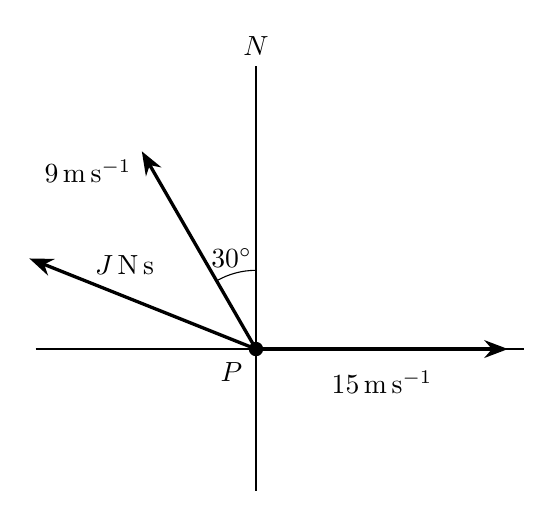
\begin{tikzpicture}[scale=2, >=Stealth]
        \coordinate (P) at (0,0);

        \pgfmathsetmacro{\angV}{120} % bearing 330° = 30° west of north
        \pgfmathsetmacro{\angJ}{180 - atan((9*sin(60))/(15 + 9*cos(60)))}

        \draw[thin] (-1.4,0) -- (1.7,0);
        \draw[thin] (0,-0.9) -- (0,1.8);
        \node[above] at (0,1.8) {$N$};

        \draw[very thick, -{Stealth[length=3mm]}]
            (P) -- (1.6,0)
            node[midway, below=4pt] {$15\,\mathrm{m\,s^{-1}}$};

        \draw[very thick, -{Stealth[length=3mm]}]
            (P) -- (\angV:1.45)
            node[pos=0.9, left=4pt] {$9\,\mathrm{m\,s^{-1}}$};

        \draw[very thick, -{Stealth[length=3mm]}]
            (P) -- (\angJ:1.55)
            node[pos=0.58, above=4pt] {$J\,\mathrm{N\,s}$};

        \fill (P) circle (1.3pt);
        \node[below left=2pt] at (P) {$P$};

        \coordinate (Ndir) at (0,1.5);
        \coordinate (Vdir) at (\angV:1.5);
        \pic[
            draw,
            angle radius=10mm,
            angle eccentricity=1.2,
            "$30^\circ$"
        ] {angle = Ndir--P--Vdir};
    \end{tikzpicture}
\end{figure}


A particle $P$ of mass $0.4\,\mathrm{kg}$ is moving due east with speed $15\,\mathrm{m\,s^{-1}}$ on a smooth horizontal plane. The particle receives a horizontal impulse of magnitude $J\,\mathrm{N\,s}$. \\

Immediately afterwards, $P$ is moving with speed $9\,\mathrm{m\,s^{-1}}$ on a bearing of $330^\circ$, as shown in the diagram. \\

Find the value of $J$ \marks{6}

\vspace*{10pt}

\begin{tcolorbox}[colback=white, colframe=scarlet, title={\textbf{Solution}}, breakable, grow to left by=6mm, grow to right by=10mm]
Use the impulse--momentum relation:
\[
\text{impulse}=\text{change in momentum}
\]

Take east as the positive \(x\)-direction and north as the positive \(y\)-direction.

Initially, the particle is moving due east at \(15\,\mathrm{m\,s^{-1}}\), so its initial velocity is
\[
\mathbf{u}=\begin{pmatrix}15\\0\end{pmatrix}
\]
Hence the initial momentum is
\[
\mathbf{p}_1=0.4\mathbf{u}
=0.4\begin{pmatrix}15\\0\end{pmatrix}
=\begin{pmatrix}6\\0\end{pmatrix}
\]

After the impulse, the particle moves with speed \(9\,\mathrm{m\,s^{-1}}\) on a bearing of \(330^\circ\).

A bearing of \(330^\circ\) means \(30^\circ\) west of north, so the final velocity has components
\[
\mathbf{v}=
\begin{pmatrix}
-9\sin30^\circ\\[2mm]
9\cos30^\circ
\end{pmatrix}
=
\begin{pmatrix}
-\frac{9}{2}\\[2mm]
\frac{9\sqrt3}{2}
\end{pmatrix}
\]
Therefore the final momentum is
\[
\mathbf{p}_2=0.4\mathbf{v}
=0.4\begin{pmatrix}
-\frac{9}{2}\\[2mm]
\frac{9\sqrt3}{2}
\end{pmatrix}
=
\begin{pmatrix}
-\frac{9}{5}\\[2mm]
\frac{9\sqrt3}{5}
\end{pmatrix}
=
\begin{pmatrix}
-1.8\\
1.8\sqrt3
\end{pmatrix}
\]

So the impulse vector is
\[
\mathbf{J}=\mathbf{p}_2-\mathbf{p}_1
=
\begin{pmatrix}
-\frac{9}{5}\\[2mm]
\frac{9\sqrt3}{5}
\end{pmatrix}
-
\begin{pmatrix}
6\\0
\end{pmatrix}
=
\begin{pmatrix}
-\frac{39}{5}\\[2mm]
\frac{9\sqrt3}{5}
\end{pmatrix}
\]

Its magnitude is
\begin{align*}
J&=\left|\mathbf{J}\right|\\
&=\sqrt{\left(-\frac{39}{5}\right)^2+\left(\frac{9\sqrt3}{5}\right)^2}\\
&=\sqrt{\frac{1521}{25}+\frac{243}{25}}\\
&=\sqrt{\frac{1764}{25}}\\
&=\frac{42}{5}
\end{align*}
Hence
\[
J=8.4\,\mathrm{N\,s}
\]

So the value of the impulse is \(8.4\,\mathrm{N\,s}\).
\end{tcolorbox}


\newpage

% ---- Question 4 ----
\questionitem
% [Source: _QBT__Vector_Momentum_and_Impulse, Q4]

A particle $Q$ of mass $0.5\,\mathrm{kg}$ is moving on a smooth horizontal surface with speed $10\,\mathrm{m\,s^{-1}}$ in the direction of the vector $4\mathbf{i}-3\mathbf{j}$. The particle then receives an impulse of magnitude $5\,\mathrm{N\,s}$ in the direction of the vector $3\mathbf{i}+4\mathbf{j}$. \\

\begin{enumerate}[label=\textbf{(\alph*)}]
  \item Find the speed of $Q$ immediately after receiving the impulse \marks{4} \\
\end{enumerate}
As a result of receiving the impulse, the direction of motion of $Q$ is turned through an angle $\theta^\circ$. \\
\begin{enumerate}[label=\textbf{(\alph*)}, resume]
  \item Find the value of $\theta$ \marks{2} \\
\end{enumerate}

\vspace*{10pt}

\begin{tcolorbox}[colback=white, colframe=scarlet, title={\textbf{Solution}}, breakable, grow to left by=6mm, grow to right by=10mm]
\begin{enumerate}[label=\textbf{(\alph*)}]
  \item The given direction vector for the initial motion is $4\mathbf{i}-3\mathbf{j}$, whose magnitude is
\[
\sqrt{4^2+(-3)^2}=5
\]
So the unit vector in this direction is
\[
\frac{4\mathbf{i}-3\mathbf{j}}{5}
\]
Hence the initial velocity is
\begin{align*}
\mathbf{v}_1
&=10\left(\frac{4\mathbf{i}-3\mathbf{j}}{5}\right) \\
&=8\mathbf{i}-6\mathbf{j}
\end{align*}

Since the mass is $0.5\,\mathrm{kg}$, the initial momentum is
\begin{align*}
\mathbf{p}_1
&=0.5(8\mathbf{i}-6\mathbf{j}) \\
&=4\mathbf{i}-3\mathbf{j}
\end{align*}

The impulse has magnitude $5\,\mathrm{N}\,\mathrm{s}$ in the direction $3\mathbf{i}+4\mathbf{j}$.
Since
\[
\lvert 3\mathbf{i}+4\mathbf{j}\rvert=5
\]
the unit vector in this direction is
\[
\frac{3\mathbf{i}+4\mathbf{j}}{5}
\]
So the impulse vector is
\begin{align*}
\mathbf{J}
&=5\left(\frac{3\mathbf{i}+4\mathbf{j}}{5}\right) \\
&=3\mathbf{i}+4\mathbf{j}
\end{align*}

Using
\[
\text{impulse}=\text{change in momentum}
\]
the final momentum is
\begin{align*}
\mathbf{p}_2
&=\mathbf{p}_1+\mathbf{J} \\
&=(4\mathbf{i}-3\mathbf{j})+(3\mathbf{i}+4\mathbf{j}) \\
&=7\mathbf{i}+\mathbf{j}
\end{align*}

Hence the final velocity is
\begin{align*}
\mathbf{v}_2
&=\frac{\mathbf{p}_2}{0.5} \\
&=\frac{7\mathbf{i}+\mathbf{j}}{0.5} \\
&=14\mathbf{i}+2\mathbf{j}
\end{align*}

Therefore the speed immediately after the impulse is
\begin{align*}
\lvert \mathbf{v}_2\rvert
&=\sqrt{14^2+2^2} \\
&=\sqrt{196+4} \\
&=\sqrt{200} \\
&=10\sqrt{2}
\end{align*}

So the speed is $10\sqrt{2}\,\mathrm{m}\,\mathrm{s}^{-1}$.

  \item The angle turned is the angle between the initial and final directions of motion.

We can use the initial direction vector $4\mathbf{i}-3\mathbf{j}$ and the final direction vector $7\mathbf{i}+\mathbf{j}$.

Using the scalar product,
\[
\cos\theta=\frac{(4,-3)\cdot(7,1)}{\lvert(4,-3)\rvert\lvert(7,1)\rvert}
\]

Now
\begin{align*}
(4,-3)\cdot(7,1)&=4\cdot 7+(-3)\cdot 1=28-3=25 \\
\lvert(4,-3)\rvert&=5 \\
\lvert(7,1)\rvert&=\sqrt{7^2+1^2}=\sqrt{50}=5\sqrt{2}
\end{align*}

So
\begin{align*}
\cos\theta
&=\frac{25}{5(5\sqrt{2})} \\
&=\frac{1}{\sqrt{2}}
\end{align*}

Hence
\[
\theta=45^\circ
\]

So the direction is turned through $45^\circ$.
\end{enumerate}
\end{tcolorbox}


\newpage

% ---- Question 5 ----
\questionitem
% [Source: _QBT__Vector_Momentum_and_Impulse, Q5]

A particle $P$ of mass $1\,\mathrm{kg}$ is moving with velocity $(3\mathbf{i}+\mathbf{j}+\mathbf{k})\,\mathrm{m\,s^{-1}}$. \\

The particle receives an impulse $\lambda(2\mathbf{i}+\mathbf{j}+2\mathbf{k})\,\mathrm{N\,s}$, where $\lambda$ is a constant. \\

Immediately after receiving the impulse, the kinetic energy of $P$ is $19\,\mathrm{J}$. \\

Find the possible values of $\lambda$ \marks{7}

\vspace*{10pt}

\begin{tcolorbox}[colback=white, colframe=scarlet, title={\textbf{Solution}}, breakable, grow to left by=6mm, grow to right by=10mm]
Impulse $=$ change in momentum.

Since the mass of $P$ is $1\,\mathrm{kg}$, its initial momentum is
\[
1(3\mathbf{i}+\mathbf{j}+\mathbf{k})=(3\mathbf{i}+\mathbf{j}+\mathbf{k})\,\mathrm{kg\,m\,s^{-1}}
\]

The impulse is
\[
\lambda(2\mathbf{i}+\mathbf{j}+2\mathbf{k})\,\mathrm{N\,s}
\]

So the momentum immediately after the impulse is
\[
(3\mathbf{i}+\mathbf{j}+\mathbf{k})+\lambda(2\mathbf{i}+\mathbf{j}+2\mathbf{k})
\]

As the mass is $1\,\mathrm{kg}$, the velocity immediately after the impulse is
\[
\mathbf{v}=(3+2\lambda)\mathbf{i}+(1+\lambda)\mathbf{j}+(1+2\lambda)\mathbf{k}
\]

The kinetic energy after the impulse is $19\,\mathrm{J}$, so
\[
\frac12(1)\lvert \mathbf{v}\rvert^2=19
\]
hence
\[
\lvert \mathbf{v}\rvert^2=38
\]

Now
\[
\lvert \mathbf{v}\rvert^2=(3+2\lambda)^2+(1+\lambda)^2+(1+2\lambda)^2
\]

So
\begin{align*}
(3+2\lambda)^2+(1+\lambda)^2+(1+2\lambda)^2&=38 \\
(9+12\lambda+4\lambda^2)+(1+2\lambda+\lambda^2)+(1+4\lambda+4\lambda^2)&=38 \\
11+18\lambda+9\lambda^2&=38
\end{align*}

Therefore
\begin{align*}
9\lambda^2+18\lambda-27&=0 \\
\lambda^2+2\lambda-3&=0 \\
(\lambda+3)(\lambda-1)&=0
\end{align*}

Hence the possible values of $\lambda$ are
\[
\lambda=1 \quad \text{or} \quad \lambda=-3
\]
\end{tcolorbox}


\newpage

% ---- Question 6 ----
\questionitem
% [Source: _QBT__Vector_Momentum_and_Impulse, Q6]

A particle $P$ of mass $5\,\mathrm{kg}$ is moving with speed $13\,\mathrm{m\,s^{-1}}$ in the direction of the vector $5\mathbf{i}-12\mathbf{j}$ when it receives an impulse $(45\mathbf{i}+90\mathbf{j})\,\mathrm{N\,s}$. \\

\begin{enumerate}[label=\textbf{(\alph*)}]
  \item Find the speed of $P$ immediately after receiving the impulse \marks{4} \\
\end{enumerate}
The direction of motion of $P$ is then changed by $\alpha^\circ$. \\
\begin{enumerate}[label=\textbf{(\alph*)}, resume]
  \item Find the value of $\alpha$ \marks{2} \\
\end{enumerate}

\vspace*{10pt}

\begin{tcolorbox}[colback=white, colframe=scarlet, title={\textbf{Solution}}, breakable, grow to left by=6mm, grow to right by=10mm]
\begin{enumerate}[label=\textbf{(\alph*)}]
  \item The given direction vector is $5\mathbf{i}-12\mathbf{j}$, whose magnitude is
  \[
  \sqrt{5^2+(-12)^2}=\sqrt{25+144}=13
  \]
  Since the speed is $13\,\mathrm{m}\,\mathrm{s}^{-1}$, the initial velocity is
  \[
  \mathbf{v}_1=13\cdot \frac{5\mathbf{i}-12\mathbf{j}}{13}=5\mathbf{i}-12\mathbf{j}
  \]
  So the initial momentum is
  \[
  \mathbf{p}_1=5\mathbf{v}_1=5(5\mathbf{i}-12\mathbf{j})=25\mathbf{i}-60\mathbf{j}
  \]

  Impulse $=$ change in momentum, so
  \[
  \mathbf{p}_2=\mathbf{p}_1+(45\mathbf{i}+90\mathbf{j})
  \]
  Hence
  \[
  \mathbf{p}_2=(25\mathbf{i}-60\mathbf{j})+(45\mathbf{i}+90\mathbf{j})
  =70\mathbf{i}+30\mathbf{j}
  \]

  Therefore the final velocity is
  \[
  \mathbf{v}_2=\frac{\mathbf{p}_2}{5}
  =\frac{70\mathbf{i}+30\mathbf{j}}{5}
  =14\mathbf{i}+6\mathbf{j}
  \]

  So the speed immediately after the impulse is
  \[
  |\mathbf{v}_2|=\sqrt{14^2+6^2}
  =\sqrt{196+36}
  =\sqrt{232}
  =2\sqrt{58}
  \]

  Therefore the speed is $2\sqrt{58}\,\mathrm{m}\,\mathrm{s}^{-1}$, approximately $15.2\,\mathrm{m}\,\mathrm{s}^{-1}$.

  \item The angle $\alpha$ is the angle between the initial and final directions, so use the scalar product of the velocity vectors:
  \[
  \mathbf{v}_1=5\mathbf{i}-12\mathbf{j},
  \qquad
  \mathbf{v}_2=14\mathbf{i}+6\mathbf{j}
  \]

  Now
  \[
  \mathbf{v}_1\cdot \mathbf{v}_2=(5)(14)+(-12)(6)=70-72=-2
  \]
  Also,
  \[
  |\mathbf{v}_1|=13,
  \qquad
  |\mathbf{v}_2|=2\sqrt{58}
  \]

  Using
  \[
  \mathbf{v}_1\cdot \mathbf{v}_2=|\mathbf{v}_1||\mathbf{v}_2|\cos\alpha
  \]
  gives
  \[
  -2=(13)(2\sqrt{58})\cos\alpha
  \]
  so
  \[
  \cos\alpha=\frac{-2}{26\sqrt{58}}=-\frac{1}{13\sqrt{58}}
  \]

  Hence
  \[
  \alpha=\cos^{-1}\!\left(-\frac{1}{13\sqrt{58}}\right)\approx 90.6^\circ
  \]

  Therefore $\alpha=\cos^{-1}\!\left(-\frac{1}{13\sqrt{58}}\right)\approx 90.6^\circ$.
\end{enumerate}
\end{tcolorbox}


\newpage

% ---- Question 7 ----
\questionitem
% [Source: _QBT__Vector_Momentum_and_Impulse, Q7]

A particle of mass $1\,\mathrm{kg}$ is moving with velocity $(\mathbf{i}+3\mathbf{j}-\mathbf{k})\,\mathrm{m\,s^{-1}}$ when it receives an impulse $\mathbf{I}\,\mathrm{N\,s}$. \\

As a result, its kinetic energy increases by $6.5\,\mathrm{J}$ and the particle then moves in the direction $(\mathbf{i}+2\mathbf{j}+\mathbf{k})$. \\

Find $\mathbf{I}$ \marks{7}

\vspace*{10pt}

\begin{tcolorbox}[colback=white, colframe=scarlet, title={\textbf{Solution}}, breakable, grow to left by=6mm, grow to right by=10mm]
Let the initial velocity be
\[
\mathbf{u}=\mathbf{i}+3\mathbf{j}-\mathbf{k}
\]

Since the mass is \(1\,\mathrm{kg}\), the initial kinetic energy is
\[
\frac12 |\mathbf{u}|^2
\]

Now
\begin{align*}
|\mathbf{u}|^2&=1^2+3^2+(-1)^2\\
&=1+9+1\\
&=11
\end{align*}

So the initial kinetic energy is
\[
\frac12 \times 11=\frac{11}{2}\text{ J}
\]

The kinetic energy increases by \(6.5\,\mathrm{J}=\dfrac{13}{2}\,\mathrm{J}\), so the final kinetic energy is
\begin{align*}
\frac{11}{2}+\frac{13}{2}&=\frac{24}{2}\\
&=12\text{ J}
\end{align*}

If \(\mathbf{v}\) is the final velocity, then
\[
\frac12 |\mathbf{v}|^2=12
\]
so
\[
|\mathbf{v}|^2=24
\]

We are told the particle then moves in the direction \((\mathbf{i}+2\mathbf{j}+\mathbf{k})\), so
\[
\mathbf{v}=\lambda(\mathbf{i}+2\mathbf{j}+\mathbf{k})
\]
for some positive scalar \(\lambda\).

Hence
\begin{align*}
|\mathbf{v}|^2&=\lambda^2(1^2+2^2+1^2)\\
&=\lambda^2(6)
\end{align*}

But \( |\mathbf{v}|^2=24\), so
\begin{align*}
6\lambda^2&=24\\
\lambda^2&=4
\end{align*}
Since the motion is in the direction \((1,2,1)\), we take \(\lambda=2\).

Therefore
\[
\mathbf{v}=2(\mathbf{i}+2\mathbf{j}+\mathbf{k})=2\mathbf{i}+4\mathbf{j}+2\mathbf{k}
\]

Impulse equals change in momentum:
\[
\mathbf{I}=m(\mathbf{v}-\mathbf{u})
\]
and since \(m=1\),
\[
\mathbf{I}=\mathbf{v}-\mathbf{u}
\]

So
\begin{align*}
\mathbf{I}&=(2\mathbf{i}+4\mathbf{j}+2\mathbf{k})-(\mathbf{i}+3\mathbf{j}-\mathbf{k})\\
&=\mathbf{i}+\mathbf{j}+3\mathbf{k}
\end{align*}

Hence the impulse is
\[
\mathbf{I}=\mathbf{i}+\mathbf{j}+3\mathbf{k}\ \mathrm{N\,s}
\]
\end{tcolorbox}


\newpage

% ---- Question 8 ----
\questionitem
% [Source: _QBT__Vector_Momentum_and_Impulse, Q8]

A particle of mass $0.8\,\mathrm{kg}$ is moving with speed $5\,\mathrm{m\,s^{-1}}$ in the direction of the vector $3\mathbf{i}+4\mathbf{j}$. It is then acted on by a constant force of $(8\mathbf{i}-6\mathbf{j})\,\mathrm{N}$ for $0.4\,\mathrm{s}$. \\

\begin{enumerate}[label=\textbf{(\alph*)}]
  \item Find the speed of the particle at the end of the $0.4\,\mathrm{s}$ interval \marks{5} \\
  \item Find the size of the angle between the direction of motion of the particle before the force acts and the direction of motion of the particle at the end of the $0.4\,\mathrm{s}$ interval \marks{3} \\
\end{enumerate}

\vspace*{1pt}

\begin{tcolorbox}[colback=white, colframe=scarlet, title={\textbf{Solution}}, breakable, grow to left by=6mm, grow to right by=10mm]
\begin{enumerate}[label=\textbf{(\alph*)}]
  \item The given direction vector is $3\mathbf{i}+4\mathbf{j}$, whose magnitude is
  \[
  \sqrt{3^2+4^2}=5
  \]

  So the initial velocity is
  \[
  \mathbf{u}=5\left(\frac{3\mathbf{i}+4\mathbf{j}}{5}\right)=3\mathbf{i}+4\mathbf{j}
  \]

  Using $\mathbf{F}=m\mathbf{a}$, the acceleration is
  \[
  \mathbf{a}=\frac{8\mathbf{i}-6\mathbf{j}}{0.8}=10\mathbf{i}-7.5\mathbf{j}
  \]

  Since the force acts for $0.4\ \mathrm{s}$, the change in velocity is
  \[
  \mathbf{a}t=(10\mathbf{i}-7.5\mathbf{j})(0.4)=4\mathbf{i}-3\mathbf{j}
  \]

  Hence the final velocity is
  \begin{align*}
  \mathbf{v}
  &=\mathbf{u}+\mathbf{a}t \\
  &=(3\mathbf{i}+4\mathbf{j})+(4\mathbf{i}-3\mathbf{j}) \\
  &=7\mathbf{i}+\mathbf{j}
  \end{align*}

  Therefore the final speed is
  \[
  |\mathbf{v}|=\sqrt{7^2+1^2}=\sqrt{50}=5\sqrt{2}
  \]

  So the speed at the end of the interval is $5\sqrt{2}\ \mathrm{m\,s^{-1}} \approx 7.07\ \mathrm{m\,s^{-1}}$.

  \item The angle between the two directions of motion is the angle between the initial and final velocity vectors.

  Initial velocity:
  \[
  \mathbf{u}=3\mathbf{i}+4\mathbf{j}
  \]

  Final velocity:
  \[
  \mathbf{v}=7\mathbf{i}+\mathbf{j}
  \]

  Using the scalar product formula,
  \[
  \cos\theta=\frac{\mathbf{u}\cdot\mathbf{v}}{|\mathbf{u}||\mathbf{v}|}
  \]

  Now
  \begin{align*}
  \mathbf{u}\cdot\mathbf{v}
  &= (3)(7)+(4)(1) \\
  &= 25
  \end{align*}

  Also,
  \[
  |\mathbf{u}|=5, \qquad |\mathbf{v}|=\sqrt{50}=5\sqrt{2}
  \]

  So
  \begin{align*}
  \cos\theta
  &=\frac{25}{5\cdot 5\sqrt{2}} \\
  &=\frac{1}{\sqrt{2}}
  \end{align*}

  Hence
  \[
  \theta=45^\circ
  \]
\end{enumerate}
\end{tcolorbox}


\end{enumerate}
\end{document}
